\section{Мета роботи}
Отримати практичні навички та закріпити знання про можливі
подання даних типу рядок та про операції над рядками.

\section{Хід роботи}
Написати програму, в якій передбачити виконання вказаної операції над рядками за умови подання рядків у пам’яті двома способами. 
Порівняти подання рядків вказаними способами за такими показниками:

\begin{itemize}
  \item обсягом використовуваної пам’яті.
	\item часом виконання функції.
\end{itemize}

Операцію та способи подання рядків вибрати з таблиці 6.1.\\

\textbf{Моє завдання:}
\begin{enumerate}
  \item Подання рядка: \textit{Блочно-зв’язне подання із змінною довжиною.}
  \item Подання рядка: \textit{Вектор з керованою довжиною рядка (з дескриптором).}
	\item Функція: \textit{Визначити кількість слів завдовжки k символів у рядку s.}
\end{enumerate}

\clearpage
\subsection{Реалізація блочно-зв’язного подання із змінною довжиною}
Дана структура даних була побудована на базі з`вязного списку та має схожу з ним реалізацію.
	Було реалізовано такі методи: \textit{ініціалізація рядка, дадовання символів у рядок, 
вивід рядка, геттер повної парснутої строки, знищення рядка.}

\begin{lstlisting}[style=customc]
#include <stdio.h>
#include <stdlib.h>
#include <string.h>

#define BLOCK_SIZE 8

typedef struct Block {
  char data[BLOCK_SIZE];
  int filled;
  struct Block *next;
} Block;

typedef struct {
  Block *head;
  Block *tail;
  size_t length;
  size_t size;
} BlockString;

BlockString *init_block_string() {
  BlockString *str = (BlockString *)malloc(sizeof(BlockString));
  if (str) {
    str->head = str->tail = NULL;
    str->length = 0;
    str->size = sizeof(BlockString);
  }
  return str;
}

void append_to_block_string(BlockString *str, const char *text) {
  size_t textLength = strlen(text);
  size_t i = 0;

  while (i < textLength) {
    if (!str->tail || str->tail->filled == BLOCK_SIZE) {

      Block *newBlock = (Block *)malloc(sizeof(Block));
      if (!newBlock)
        return;
      memset(newBlock->data, '\0', BLOCK_SIZE);
      newBlock->filled = 0;
      newBlock->next = NULL;

      if (str->tail) {
        str->tail->next = newBlock;
      } else {
        str->head = newBlock;
      }
      str->tail = newBlock;

      str->size += sizeof(Block);
    }

    while (i < textLength && str->tail->filled < BLOCK_SIZE) {
      str->tail->data[str->tail->filled++] = text[i++];
      str->length++;
    }
  }
}

char *get_block_string(BlockString *str) {
  char *result = malloc((str->length + 1) * sizeof(char));
  Block *current = str->head;
  size_t i = 0;

  while (current) {
    strncpy(result + i, current->data, current->filled);
    i += current->filled;
    current = current->next;
  }
  result[str->length] = '\0';
  return result;
}

void print_block_string(BlockString *str) {
  Block *current = str->head;
  printf("String: ");
  while (current) {
    for (int i = 0; i < current->filled; i++) {
      putchar(current->data[i]);
    }
    current = current->next;
  }
  printf("\n");
  printf("Length: %zu\n", str->length);
  printf("Total size: %zu bytes\n", str->size);
}

void destroy_block_string(BlockString *str) {
  Block *current = str->head;
  while (current) {
    Block *next = current->next;
    free(current);
    current = next;
  }
  free(str);
}
\end{lstlisting}

\clearpage
\subsection{Реалізація вектора з керованою довжиною рядка}

	Було реалізовано такі методи: \textit{ініціалізація рядка, дадовання символів у рядок, 
вивід рядка, знищення рядка.}
  
\begin{lstlisting}[style=customc]
#include <stdio.h>
#include <stdlib.h>
#include <string.h>

typedef struct {
  char *data;
  size_t length;
  size_t capacity;
  size_t size;
} VectorString;

VectorString *init_vector_string(size_t capacity) {
  VectorString *str = (VectorString *)malloc(sizeof(VectorString));
  if (!str) {
    printf("Error: Memory allocation failed.\n");
    return NULL;
  }

  str->data = (char *)malloc(capacity * sizeof(char));
  if (str->data) {
    str->length = 0;
    str->capacity = capacity;
    str->size = sizeof(VectorString) + capacity;
    str->data[0] = '\0';
  } else {
    free(str);
    return NULL;
  }

  return str;
}

void append_to_vector_string(VectorString *str, const char *text) {
  size_t newLength = str->length + strlen(text);
  if (newLength >= str->capacity) {
    size_t newCapacity = newLength * 2;
    char *newData = (char *)realloc(str->data, newCapacity * sizeof(char));
    if (!newData) {
      printf("Error: Memory reallocation failed.\n");
      return;
    }
    str->data = newData;
    str->capacity = newCapacity;
    str->size = sizeof(VectorString) + newCapacity;
  }

  strcat(str->data, text);
  str->length = newLength;
}

void print_vector_string(const VectorString *str) {
  printf("String: %s\n", str->data);
  printf("Length: %zu\n", str->length);
  printf("Capacity: %zu\n", str->capacity);
  printf("Total size: %zu bytes\n", str->size);
}

void destroy_vector_string(VectorString *str) {
  free(str->data);
  free(str);
}

\end{lstlisting}

\subsection{Основна програма з заданою функцією та результатами порівняння:}
Реалізація функції для визначення кількості слів завдовжки k символів у рядку:

\begin{lstlisting}[style=customc]
int countWordsOfLengthK(const char *str, size_t k) {
  int count = 0;
  size_t wordLength = 0;
  const char *s = str;

  while (*s) {
    if (isalpha(*s)) {
      wordLength++;
    } else {
      if (wordLength == k) {
        count++;
      }
      wordLength = 0;
    }
    s++;
  }

  if (wordLength == k) {
    count++;
  }

  return count;
}
\end{lstlisting}

Реалізація функції тестування на зайняту пам`ять та швидкість роботи функції пошуку слів.
Вона приймає строку яка буде додана до структури та кількість повторних занесень цієї строки до структури для створення навантаження.

\begin{lstlisting}[style=customc]
double measureExecutionTime(int (*func)(const char *, size_t), const char *str,
                            size_t k) {
  clock_t start = clock();
  func(str, k);
  return ((double)(clock() - start) / CLOCKS_PER_SEC) * 1000;
}

void benchmark(const char *str, int dublicates) {
  int k = 3; // searching words length

  BlockString *blockStr = init_block_string();
  VectorString *vectorStr = init_vector_string(10);

  for (int i = 0; i < dublicates; i++) {
    append_to_vector_string(vectorStr, str);
    append_to_block_string(blockStr, str);
  }

  char *parsedBlockStr = get_block_string(blockStr);

  double vectorTime =
      measureExecutionTime(countWordsOfLengthK, vectorStr->data, k);
  double blockTime =
      measureExecutionTime(countWordsOfLengthK, parsedBlockStr, k);

  printf("\nWord count of length %zu in vector string: %d\n", k,
         countWordsOfLengthK(vectorStr->data, k));
  printf(
      "Execution time \033[34m(vector string)\033[0m: \033[32m%.2f ms\033[0m\n",
      vectorTime);
  printf("Memory used: \033[32m%zu bytes\033[0m\n", vectorStr->size);

  printf("\nWord count of length %zu in block string: %d\n", k,
         countWordsOfLengthK(parsedBlockStr, k));
  printf(
      "Execution time \033[34m(block string)\033[0m: \033[32m%.2f ms\033[0m\n",
      blockTime);
  printf("Memory used: \033[32m%zu bytes\033[0m\n\n", blockStr->size);

  free(parsedBlockStr);
  destroy_block_string(blockStr);
  destroy_vector_string(vectorStr);
}
\end{lstlisting}

Реалізація функції main:

\begin{lstlisting}[style=customc]
void task1() {
  int k = 3;
  BlockString *blockStr = init_block_string();
  VectorString *vectorStr = init_vector_string(10);

  highlightText("VECTOR STRING IMPLEMENTATION", "blue");

  append_to_vector_string(vectorStr, "Glory ");
  append_to_vector_string(vectorStr, "to ");
  append_to_vector_string(vectorStr, "Ukraine");
  append_to_vector_string(vectorStr, "!");

  print_vector_string(vectorStr);

  printf("\n");
  highlightText("BLOCK-LINKED STRING IMPLEMENTATION", "blue");

  append_to_block_string(blockStr, "Glory ");
  append_to_block_string(blockStr, "to ");
  append_to_block_string(blockStr, "Ukraine");
  append_to_block_string(blockStr, "!");

  print_block_string(blockStr);

  printf("\n");
  highlightText("MEMORY AND ESTIMATE TIME TEST OF STRING DATA STRUCTURES",
                "blue");

  benchmark("Cat was sad but ate pie. ", 1000);
  puts("-------------------------------------------");
  benchmark("Cat was sad but ate pie. ", 10000);
  puts("-------------------------------------------");
  benchmark("Cat was sad but ate pie. ", 100000);

  destroy_block_string(blockStr);
  destroy_vector_string(vectorStr);
}
\end{lstlisting}


\subsection{Результати роботи програми:}
Просте занесення рядків до структур та вивід інформації про них:

\begin{figure}[h!]
    \centering
    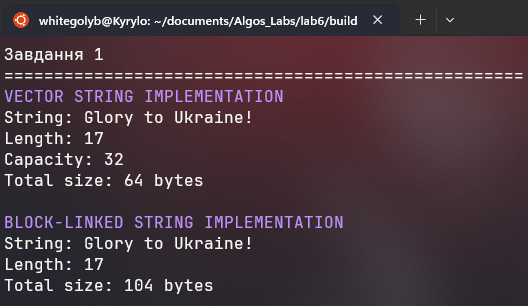
\includegraphics[width=15cm]{reports/algos/lab6/assets/1.png}
    \caption{Тестовий вивід рядків з заповненими кусочно рядками}
\end{figure}

\clearpage
Результати стресс-тестування структур даних з різною кількостю дублікатів задних рядків:

\begin{figure}[h!]
  \centering
  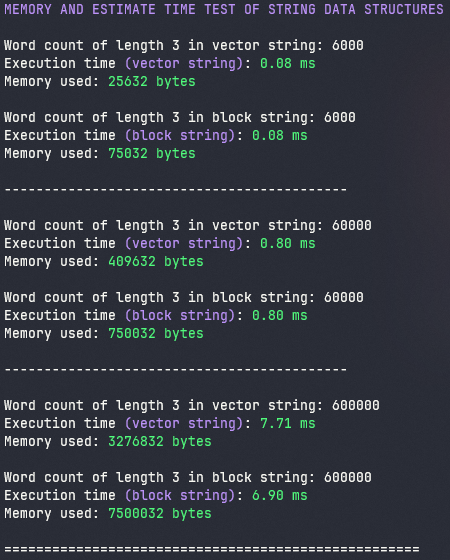
\includegraphics[width=15cm]{reports/algos/lab6/assets/2.png}
  \caption{Результати стресс-тестів}
\end{figure}

\clearpage
\section{Висновки}
  В ході виконання лабораторної роботи було розроблено дві структури даних відповідно свого
варіанту та відповідну функцію пошуку слів вказаної довжини.\\

  Подивившись на отримані результати тестування можна зазначити що структура даних 
блочно-зв`язного типу займає більше місця у ОЗУ ніж структура рядка векторного типу (майже в два рази більше). Така різниця обумовлена тим що  блочно-зв`язна струтрура розроблена на базі зв`язного списку для вузлів якого виділяється додаткова пам`ять щоб їх зберігати та кожна нова строка створює новий вузол певного розміру. Тим часов векторна структура просто оновлює розмір неперервної ділянки пам`яті у два рази незалежно від довжини нового доданого рядка.\\

  Результати тестування швидкості роботи функції майже не відрізняються на малих рядках, проте
якщо довжина рядку буде збільшуватися, то функція буде працювати трішки швидше зі блочно-зв`язною структурою що можна побачити з останнього результату.



